\chapter{Introduction}

Device driver synthesis has been proposed as a radical alternative to traditional driver development that offers the promise of creating drivers faster and with far fewer defects~\cite{Ryzhyk_CKSH_09}. The idea is to automatically generate the driver code responsible for controlling device operations from a behavioural model of the device and a specification of the driver-OS interface.

The primary motivations for device driver synthesis are the fact that device drivers are hard and tedious to write, and they are notorious for being unreliable~\cite{Chou_YCHE_01,Ganapathi_GP_06}. Drivers generally take a long time to bring to production---given the speed at which new devices can be brought to market today, it is not uncommon for a device release to be delayed by driver rather than by silicon issues~\cite{Yavatkar_12}. 

Automatic driver synthesis was proposed in earlier work on the Termite-1 project~\cite{Ryzhyk_CKSH_09}, which formulated the key principles behind the approach and demonstrated its feasibility by synthesising drivers for several real-world devices.  The next logical step was to develop driver synthesis into a practical methodology, capable of replacing the conventional driver development process.  To this end, this thesis addresses the key problems left open by Termite-1:

\begin{itemize}
    \item Termite-1 produced poor quality synthesised code.  While functionally correct, Termite-1 drivers were bloated and poorly structured.  This made it impossible for a programmer to maintain and improve the generated code and prevented synthesised drivers from being adopted by Linux and other major operating systems.  Furthermore, it was impossible to enforce non-functional properties such as CPU and power efficiency. Addressing these issues is the first major contribution of this dissertation.
    \item The scalability of the Termite-1 synthesis algorithm was severely limited, which made synthesis of drivers for real-world devices intractable. Termite-1 got around the problem by using carefully crafted simplified device specifications, which is acceptable in a proof-of-concept prototype, but not in a practical tool. Addressing this issue is the second major contribution of this dissertation.
\end{itemize}

\section{Game Based Formalism}

The key step towards addressing the above challenges is to capture the driver synthesis problem using a precise mathematical formalism.  In this work, I develop the first precise mathematical formulation of the driver synthesis problem.  This enables us to apply theoretical results and algorithmic techniques from game theory to driver synthesis.  Following the approach proposed by Termite-1, I treat the driver synthesis problem as a two-player game between the driver and its environment, comprised of the device and the OS\@. Each player has a set of \emph{moves} available to it. The driver's moves are called the \emph{controllable} moves, while the environment's moves are \emph{uncontrollable}. The driver's moves, for example, may consist of the set of device register writes that it can perform. The game is played on a large state machine that describes the behaviour of the device and operating system. At any instant, one state is the \emph{current state} and play progresses from state to state by following edges labelled with the set of moves. 

However, the formal model used in Termite-1 had several important shortcomings that made it unsound, potentially leading to incorrect synthesised drivers or synthesis failures.  The \emph{objective} of a Termite-1 game was defined by designating some states as \emph{goal} states. A goal may, for example, correspond to a state where the driver has no outstanding data to send. A correct driver is defined as one that can eventually force the current state to be in the set of goal states, regardless of the environment behaviour. 

Objectives, defined using goals, are insufficient for two reasons. First, they do not capture recurring properties. Termite-1 considered a driver to be correct if it could force execution into the goal once. Real drivers, however, are reactive systems that need to continuously satisfy requests. Second, such objectives do not allow the driver to make realistic assumptions about how the environment behaves. Termite-1 drivers could not rely on simple properties like the fact that timeouts eventually time out. This is discussed further in Section~\ref{sec:game_fairness}. 

The new tool called Termite-2 (further referred to as Termite) overcomes these shortcomings by using generalised reactive (1), or GR(1) objectives \cite{Piterman_PS_06}.

In addition, Termite-1 did not handle the concurrency between the driver and its environment properly, resulting in subtly incorrect drivers. I handle this in a robust way using concurrent games. 


\section{User Guided Synthesis}

The Termite team and I came to the conclusion that the approach taken by Termite-1 was \emph{critically flawed}.  The fundamental problem, in our view, was that the synthesis was viewed as a ``push-button'' technology that generated a specification-compliant implementation without any user involvement.  As a result, the user had to rely on the synthesis tool to produce a good implementation.  Unfortunately, even the most intelligent algorithm cannot fully capture the user-perceived notion of high-quality code.  While in theory one might be able to enforce some of the desired properties by adding appropriate constraints to the input specification, in our experience creating such specifications is extremely hard and seldom yields satisfactory results.

A radically different approach was needed---one that combines the power of automation with the flexibility of conventional development, and that involves the developer from the start, guiding the generation of the driver.  In many ways, synthesis and conventional development are conflicting.  Hence, a key challenge was to conceive of a way that allowed the two to be combined so that the developer could do their job more efficiently and with fewer errors without having the synthesis tool get in the way.

This dissertation presents a novel \emph{user-guided} approach to driver synthesis implemented in Termite.  In \termite, the user has full control over the synthesis process, while the tool acts as an assistant that suggests, but does not enforce, implementation options and ensures correctness of the resulting code.  At any point during synthesis the user can modify or extend previously synthesised code.  The tool automatically analyses user-provided code and, on user's request, suggests possible ways to extend it to a complete implementation.  If such an extension is not possible due to an error in the user code, the tool generates an explanation of the failure that helps the user to identify and correct the error.

In an extreme scenario, \termite can be used to synthesise the complete implementation fully automatically.  At the other extreme, the user can build the complete implementation by hand, in which case \termite acts as a static verifier for the driver.  In practice, it was determined that the intermediate approach, where most of the code is auto-generated, but manual involvement is used when needed to improve the implementation, to be the most practical.

From the developer's perspective, user-guided synthesis appears as an enhancement of the conventional development process with very powerful autocomplete functionality, rather than a completely new development methodology. Input specifications for driver synthesis are written as imperative programs that model the behaviour of the device and the OS\@.  The driver itself is modelled as a source code template where parts to be synthesised are omitted.  This approach enables the use of familiar programming techniques in building input specifications.  In contrast, previous synthesis tools, including Termite-1, require specifications to be written in formal languages based on state machines and temporal logic, which proved difficult and error-prone to use even for formal methods experts, not to mention software development practitioners.

Most previous research on automatic synthesis, including Termite-1, considered input specifications to be ``correct by definition''.  In contrast, we recognise that input specifications produced by human developers are likely to contain defects, which can prevent the synthesis algorithm from finding a correct driver implementation.  Therefore \termite incorporates powerful debugging tools that help the developer identify and fix specification defects through well-defined steps, similar to how conventional debuggers help troubleshoot implementation errors.

Figure~\ref{f:termite_intro} gives an overview of the components of Termite and the synthesis workflow. I will be presenting each of the following components in the remaining chapters of this thesis:
\begin{itemize}
    \item A scalable synthesis algorithm.
    \item A high level specification language and compiler.
    \item A graphical debugging and state space exploration environment.
    \item A counterexample generator.
    \item A heuristic code generator.
\end{itemize}

\begin{figure}
    \center
    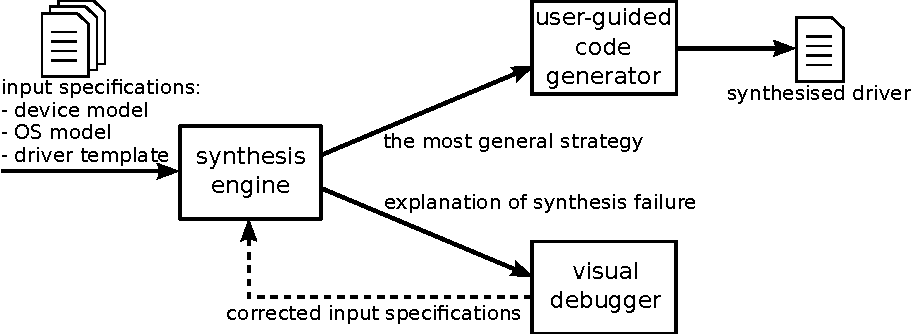
\includegraphics[width=\linewidth]{imgs/termite.pdf}
    \caption{\termite synthesis workflow.}\label{f:termite_intro}
\end{figure}

I evaluated \termite by synthesising drivers for several I/O devices representative of peripherals found in a typical embedded system. The evaluation criteria are:
\begin{itemize}
    \item Percent of the driver that is synthesiseable by Termite.
    \item Performance and code size of the synthesized driver.
    \item Synthesis algorithm running time and memory usage.
    \item Ease of creation and debugging of the specifications.
\end{itemize}
I conclude that for typical embedded devices automatic driver synthesis is practical. 

Device driver synthesis technology is still in its early days and, as such, has several important limitations.  Most notably, \termite does not currently support synthesis or verification of code for managing direct memory access (DMA) queues.  This code must be written manually and is treated by \termite as an external API invoked by the driver. This limitation makes the use of Termite less appealing for devices such as gigabit ethernet controllers where the majority of driver writing effort goes into handling DMA. As another example, in certain situations, explained in Chapter~\ref{ch:userguided} Section~\ref{s:user-guided}, \termite is unable to produce correct code without user assistance; however it is able to verify the correctness of user-provided code.  We discuss limitations of \termite in more detail in Chapter~\ref{ch:userguided} Section~\ref{s:limitations}.

This dissertation makes two contributions in the field of practical device driver synthesis:
\begin{enumerate}
    \item A practical synthesis tool that allows the user to work anywhere on the spectrum from full automation to verified manual development.
    \item A counterexample guided debugging environment that the developer may use to interactively eliminate defects in the input specifications.
\end{enumerate}

\section{Scalable Synthesis Algorithm}
\label{sec:scalable_synth}

To address the scalability problem, I created a new scalable synthesis algorithm, which mitigates the computational bottleneck in driver synthesis~\cite{Walker_Ryzhyk_14}. Our game-based synthesis algorithm relies on abstraction and symbolic reasoning to achieve orders of magnitude speed up compared to the current state-of-the-art synthesis techniques. The algorithm, along with supporting benchmarks, is given in Chapter~\ref{ch:solving}.

Game solving inherently involves exploring the state space of the game. These state spaces are potentially very large and exploring them becomes difficult. This is referred to as the state space explosion problem. \emph{Abstraction} offers an effective approach to mitigating the state space explosion problem.  For example, in the model checking domain abstraction proved instrumental in enabling automatic verification of complex hardware and software systems~\cite{Clarke_GJLV_00,Clarke_KSY_04,Henzinger_JMS_02}.  The reactive synthesis community has also identified the key role of abstraction in tackling real-world synthesis problems; however most research in this area has so far been of theoretical nature~\cite{Alfaro_Roy_07,Henzinger_JM_03}.  

In this dissertation I present the first practical abstraction-refinement algorithm for solving games.  Our algorithm is based on \emph{predicate abstraction}, which proved to be particularly successful in model checking~\cite{Graf_Saidi_97}.  Predicate abstraction partitions the state space of the game based on a set of predicates, which capture essential properties of the system.  States inside a partition are indistinguishable to the abstraction, which limits the maximal precision of solving the game achievable with the given abstraction.  The abstraction is iteratively refined by introducing new predicates.

The key difficulty in applying predicate abstraction to games is to efficiently solve the abstract game arising at every iteration of the abstraction refinement loop.  This requires computing the abstract \emph{controllable predecessor} operator, which maps a set of abstract states, winning for one of the players, into the set of states from which the player can force the game into the winning set in one round of the game.  This involves enumerating concrete moves available to both players in each abstract state, which can be prohibitively expensive.  

I address the problem by further approximating the expensive controllable predecessor computation and refining the approximation when necessary. To this end, I introduce additional predicates that partition the set of actions available to the players into \emph{abstract actions}.  The controllable predecessor computation then consists of two steps: (1) computing abstract actions available in each abstract state, and (2) evaluating controllable predecessor over abstract states and actions.  

The first step involves potentially expensive analysis of concrete transitions of the system and is therefore computed approximately.  More specifically, solving the abstract game requires overapproximating moves available to one of the players, while underapproximating moves available to the other~\cite{Henzinger_JM_03}.  The former is achieved by allowing an abstract action in an abstract state if it is available in at least one corresponding concrete state, the latter allows an action only if it is available in all corresponding concrete states.  I compute the overapproximation by initially allowing all actions in all states and gradually refining the abstraction by eliminating spurious actions.  Conversely, I start with an empty underapproximation and add available actions as necessary.

This dissertation makes three contributions in the field of reactive synthesis:
\begin{enumerate}
    \item I propose the first practical predicate-based abstraction refinement algorithm for two-player games.

    \item I introduce a new type of refinement, which increases the precision of controllable predecessor computation without refining the abstract state space of the game.  This approach avoids costly operations involved in solving the abstract game, approximating them with a sequence of light-weight operations performed on demand, leading to dramatically improved scalability.

    \item I evaluate the algorithm by implementing it as part of the Termite driver synthesis toolkit~\cite{Ryzhyk_WKLRSV_14} and using it to synthesise drivers for complex real-world devices.  Our algorithm efficiently solves games with very large state spaces, which is impossible without using abstraction or using simpler forms of abstraction.
\end{enumerate}

\section{Chapter Outline}

The rest of this dissertation is structured as follows. Chapter~\ref{ch:background} provides the necessary background information on game solving. Chapter~\ref{ch:userguided} presents our user guided device driver synthesis tool and methodology and, finally, Chapter~\ref{ch:solving} presents our scalable synthesis algorithm.
